\let\negmedspace\undefined
\let\negthickspace\undefined
\documentclass[journal]{IEEEtran}
\usepackage[a5paper, margin=10mm, onecolumn]{geometry}
%\usepackage{lmodern} % Ensure lmodern is loaded for pdflatex
\usepackage{tfrupee} % Include tfrupee package

\setlength{\headheight}{1cm} % Set the height of the header box
\setlength{\headsep}{0mm}     % Set the distance between the header box and the top of the text

\usepackage{gvv-book}
\usepackage{gvv}
\usepackage{cite}
\usepackage{amsmath,amssymb,amsfonts,amsthm}
\usepackage{algorithmic}
\usepackage{graphicx}
\usepackage{textcomp}
\usepackage{xcolor}
\usepackage{txfonts}
\usepackage{listings}
\usepackage{enumitem}
\usepackage{mathtools}
\usepackage{gensymb}
\usepackage{comment}
%\usepackage{multiclo}
\usepackage[breaklinks=true]{hyperref}
\usepackage{tkz-euclide} 
\usepackage{listings}
% \usepackage{gvv} 
\graphicspath{ {./figs/} }

\begin{document}

\title{
AE: AEROSPACE ENGINEERING}
\author{AI25BTECH11013-Gautham Pocha}
\maketitle
\renewcommand{\thefigure}{\theenumi}
\renewcommand{\thetable}{\theenumi}


\begin{enumerate}
\item Isentropic efficiency $ \eta_d $ of a subsonic diffuser is defined as 

(Note: ‘a’ represents the ambient, ‘2’ represents the exit of the diffuser and ‘s’ represents an isentropic process)
\begin{multicols}{4}
\begin{enumerate}
\item $ \frac{T_{02}}{T_0} - T_a $
\item $ \frac{T_{02} + T_a}{T_{02} + T_a} $
\item $ \frac{P_{02} - P_a}{P_0 - P_a} $
\item $ \frac{P_a - P_{02}}{P_a - P_{02}} $
\end{enumerate}
\end{multicols}
\hfill (GATE AE 2010)

\item Two position vectors are indicated by $ \vec{V}_1 = \myvec{x_1 \\ y_1} $ and $ \vec{V}_2 = \myvec{x_2 \\ y_2} $. If $ a^2 + b^2 = 1 $, then the operation $ \vec{V}_2 = \myvec{a & -b \\ b & a} \vec{V}_1 $ amounts to obtaining the position vector $ \vec{V}_2 $ from $ \vec{V}_1 $ by
\begin{enumerate}
\item translation
\item rotation
\item magnification
\item combination of translation, rotation, and magnification.
\end{enumerate}
\hfill (GATE AE 2010)

\item An aircraft is climbing at a constant speed in a straight line at a steep angle of climb. The load factor it sustains during the climb is:
\begin{multicols}{2}
\begin{enumerate}
\item equal to 1.0
\item greater than 1.0
\item positive but less than 1.0
\item dependant on the weight of the aircraft
\end{enumerate}
\end{multicols}
\hfill (GATE AE 2010)

\item In a general case of a homogeneous material under thermo-mechanical loading the number of distinct components of the state of stress is
\begin{multicols}{4}
\begin{enumerate}
\item 3
\item 4
\item 5
\item 6
\end{enumerate}
\end{multicols}
\hfill (GATE AE 2010)

\item The linear second order partial differential equation $ 5 \frac{\partial^2 \phi}{\partial x^2} + 3 \frac{\partial^2 \phi}{\partial x \partial y} + 2 \frac{\partial^2 \phi}{\partial y^2} + 9 = 0 $ is
\begin{multicols}{2}
\begin{enumerate}
\item Parabolic
\item Hyperbolic
\item Elliptic
\item None of the above
\end{enumerate}
\end{multicols}
\hfill (GATE AE 2010)

\item All other factors remaining constant, if the weight of an aircraft increases by 30\% then the takeoff distance increases by approximately:
\begin{multicols}{4}
\begin{enumerate}
\item 15\%
\item 30\%
\item 70\%
\item 105\%
\end{enumerate}
\end{multicols}
\hfill (GATE AE 2010)

\item A vertical slender rod is suspended by a hinge at the top and hangs freely. It is heated until it attains a uniform temperature, $ T $. Neglecting the effect of gravity, the rod has
\begin{multicols}{2}
\begin{enumerate}
\item Stress but no strain
\item Strain but no stress
\item Both stress and strain
\item Neither stress nor strain
\end{enumerate}
\end{multicols}
\hfill (GATE AE 2010)

\item An aircraft stalls at a speed of 40 m/s in straight and level flight. The slowest speed at which this aircraft can execute a level turn at a bank angle of 60 degrees is:
\begin{multicols}{4}
\begin{enumerate}
\item 28.3 m/s
\item 40.0 m/s
\item 56.6 m/s
\item 80.0 m/s
\end{enumerate}
\end{multicols}
\hfill (GATE AE 2010)

\item The eigen-values of a real symmetric matrix are always
\begin{multicols}{2}
\begin{enumerate}
\item positive
\item imaginary
\item real
\item complex conjugate pairs
\end{enumerate}
\end{multicols}
\hfill (GATE AE 2010)

\item The concentration $ x $ of a certain chemical species at time $ t $ in a chemical reaction is described by the differential equation $ \frac{dx}{dt} + kx = 0 $, with $ x(t = 0) = x_0 $. Given that $ e $ is the base of the natural logarithms, the concentration $ x $ at $ t = \frac{1}{k} $
\begin{multicols}{2}
\begin{enumerate}
\item falls to the value $ 0.5x_0 $
\item rises to the value $ 2x_0 $
\item falls to the value $ \frac{x_0}{e} $
\item rises to the value $ ex_0 $
\end{enumerate}
\end{multicols}
\hfill (GATE AE 2010)

\item The definite integral $ \int_{-1}^{1} \frac{dx}{x^2} $
\begin{multicols}{4}
\begin{enumerate}
\item does not exist
\item is equal to 2
\item is equal to 0
\item is equal to -2
\end{enumerate}
\end{multicols}
\hfill (GATE AE 2010)

\item The absolute ceiling of an aircraft is the altitude above which it:
\begin{enumerate}
\item can never reach
\item cannot sustain level flight at a constant speed
\item can perform accelerated flight as well as straight and level flight at a constant speed
\item can perform straight and level flight at a constant speed only
\end{enumerate}
\hfill (GATE AE 2010)

\item A thin rectangular plate made of isotropic material which satisfies the octahedral (i.e., Von Mises/ Distortion energy) failure criterion has yield strength of 200 MPa under uniaxial tension. As shown in the figure, if it is loaded with uniform tension of 150 MPa along the $ x $-direction, the maximum uniform tensile stress that can be applied along the $ y $-direction before the plate starts yielding is about 
    
\begin{figure}[H]
    \centering
    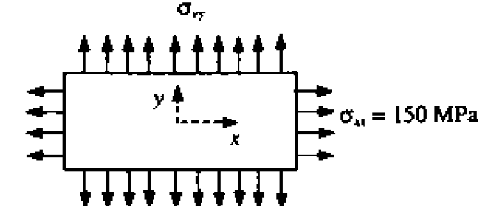
\includegraphics[width=0.6\textwidth]{1.png}
    \caption{}
    \label{fig:question13}
\end{figure}
    
\begin{multicols}{4}
\begin{enumerate}
\item 227 MPa
\item 77 MPa
\item 87 MPa
\item 114 MPa
\end{enumerate}
\end{multicols}
\hfill (GATE AE 2010)

\item Consider an incompressible 2-D Couette flow of water between two walls spaced 1m apart. The lower wall is kept stationary. What is the shear stress acting on the lower wall if the upper wall is moving at a constant speed of $ 2  \text{m/s}^2 $ ($ \mu_{\text{water}} = 7 \times 10^{-3}  \text{N.s/m}^2 $)
    
\begin{figure}[H]
    \centering
    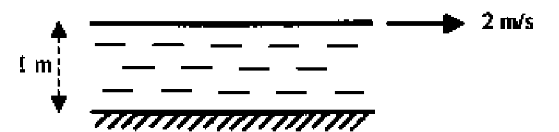
\includegraphics[width=0.6\textwidth]{2.png}
    \caption{}
    \label{fig:question14}
\end{figure}
    
\begin{multicols}{4}
\begin{enumerate}
\item $ 3.5 \times 10^{-3}  \text{N/m}^2 $
\item $ 7 \times 10^{-3}  \text{N/m}^2 $
\item $ 10.5 \times 10^{-3}  \text{N/m}^2 $
\item $ 14 \times 10^{-3}  \text{N/m}^2 $
\end{enumerate}
\end{multicols}
\hfill (GATE AE 2010)

\item The angular momentum, about the centre of mass of the earth, of an artificial satellite in a highly elliptical orbit is:
\begin{enumerate}
\item a maximum when the satellite is farthest from the earth
\item a constant
\item proportional to the speed of the satellite
\item proportional to the square of the speed of the satellite
\end{enumerate}
\hfill (GATE AE 2010)

\item A column of length $l$ and flexural rigidity $EI$ has one end fixed and the other end hinged. The critical buckling load for the column is:

\begin{multicols}{4}
\begin{enumerate}
\item $\dfrac{\pi^2 EI}{(0.5l)^2}$  
\item $\dfrac{\pi^2 EI}{(0.7l)^2}$  
\item $\dfrac{\pi^2 EI}{l^2}$  
\item $\dfrac{\pi^2 EI}{(2l)^2}$  
\end{enumerate}
\end{multicols}
\hfill (GATE AE 2010)

\item A horizontal cantilevered steel beam of rectangular cross-section having width $b$ and depth $d$ is vibrating in the vertical plane. The natural frequency of bending vibration is highest when:

\begin{figure}[H]
    \centering
    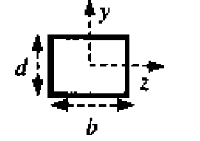
\includegraphics[width=0.6\textwidth]{3.png}
    \caption{}
    \label{fig:question17}
\end{figure}
    
\begin{multicols}{4}
\begin{enumerate}
\item $b = 10$, $d = 10$  
\item $b = 20$, $d = 5$  
\item $b = 5$, $d = 20$  
\item $b = 25$, $d = 4$  
\end{enumerate}
\end{multicols}
\hfill (GATE AE 2010)

\item Consider an incompressible 2-D viscous flow over a curved surface. Let the pressure distribution on the surface be $p(s) = 2 + \sin\left(\dfrac{\pi}{2} + s\right)$ [N/m$^2$], where $s$ is the distance along the curved surface from the leading edge. The flow separates at:

\begin{multicols}{4}
\begin{enumerate}
\item $s = \dfrac{2}{3}\pi$ m  
\item $s = \dfrac{3}{2}\pi$ m  
\item $s = \dfrac{\pi}{2}\pi$ m  
\item $s = \pi$ m  
\end{enumerate}
\end{multicols}
\hfill (GATE AE 2010)

\item For a multi-stage axial compressor with constant diameter hub:
\begin{enumerate}
\item Blade height decreases in the flow direction  
\item Blade height increases in the flow direction  
\item Blade height remains constant  
\item Blade height first increases and then decreases in the flow direction  
\end{enumerate}
\hfill (GATE AE 2010)

\item In a 2-D, steady, fully developed, laminar boundary layer over a flat plate, if $x$ is the stream-wise coordinate, $y$ is the wall normal coordinate and $u$ is the stream-wise velocity component, which of the following is true:
\begin{multicols}{4}
\begin{enumerate}
\item $\dfrac{\partial u}{\partial x} \gg \dfrac{\partial u}{\partial y}$  
\item $\dfrac{\partial u}{\partial y} \gg \dfrac{\partial u}{\partial x}$  
\item $\dfrac{\partial u}{\partial x} = \dfrac{\partial u}{\partial y}$  
\item $\dfrac{\partial u}{\partial x} = \dfrac{\partial u}{\partial y}$  
\end{enumerate}
\end{multicols}
\hfill (GATE AE 2010)

\item How does the specific thrust, at constant turbine inlet temperature, produced by a turbofan engine change with an increase in compressor pressure ratio?
\begin{multicols}{2}
\begin{enumerate}
\item Increases  
\item Decreases  
\item First increases and then decreases  
\item First decreases and then increases  
\end{enumerate}
\end{multicols}
\hfill (GATE AE 2010)

\item If $\phi$ is the potential function for an incompressible irrotational flow, and $u$ and $v$ are the Cartesian velocity components, then which one of the following combinations is correct?

\begin{multicols}{2}
\begin{enumerate}
\item $u = \dfrac{\partial \phi}{\partial x},\quad v = \dfrac{\partial \phi}{\partial y}$  
\item $u = -\dfrac{\partial \phi}{\partial x},\quad v = \dfrac{\partial \phi}{\partial y}$  
\item $u = -\dfrac{\partial \phi}{\partial y},\quad v = \dfrac{\partial \phi}{\partial x}$  
\item $u = \dfrac{\partial \phi}{\partial y},\quad v = \dfrac{\partial \phi}{\partial x}$  
\end{enumerate}
\end{multicols}
\hfill (GATE AE 2010)

\item Among the choices given below, the Specific Impulse is maximum for a:

\begin{multicols}{2}
\begin{enumerate}
\item Cryogenic Rocket  
\item Solid Rocket  
\item Liquid Rocket  
\item Hybrid Rocket  
\end{enumerate}
\end{multicols}
\hfill (GATE AE 2010)

\item For a flow across an oblique shock which of the following statements is true?
\begin{enumerate}
\item Component of velocity normal to shock decreases while tangential component increases.
\item Component of velocity normal to shock increases while tangential component decreases.
\item Component of velocity normal to shock is unchanged while tangential component decreases.
\item Component of velocity normal to shock decreases while tangential component is unchanged.
\end{enumerate}
\hfill (GATE AE 2010)

\item The maximum operating flow rate through a centrifugal compressor at a given RPM is limited by
\begin{multicols}{2}
\begin{enumerate}
\item Impellor stall
\item Surge
\item Choking of diffuser throat
\item Inlet flow distortion
\end{enumerate}
\end{multicols}
\hfill (GATE AE 2010)

\item A spacecraft of mass 100 kg, moving at an instantaneous speed of $1.8 \times 10^4  \text{m/s}$, picks up interstellar dust at the rate of $3.2 \times 10^{-8}  \text{kg/s}$. Assuming that the dust was initially at rest, the instantaneous rate of retardation of the spacecraft is:
\begin{multicols}{4}
\begin{enumerate}
\item $7.9 \times 10^{-8}  \text{m/s}^2$
\item $2.3 \times 10^{-3}  \text{m/s}^2$
\item zero
\item $5.8 \times 10^{-6}  \text{m/s}^2$
\end{enumerate}
\end{multicols}
\hfill (GATE AE 2010)

\item Following stress state is proposed for a 2-D problem with no body forces: $\sigma_{xx} = 3x^2y + 4y^2$, $\sigma_{yy} = y^3 + 14xy$, $\tau_{xy} = -3xy^2 - 7x^2$. It satisfies
\begin{enumerate}
\item Equilibrium equations but not compatibility equation
\item Compatibility equation but not equilibrium equations
\item Neither equilibrium equations nor compatibility equation
\item Both equilibrium equations and compatibility equation
\end{enumerate}
\hfill (GATE AE 2010)

\item A uniform cross-section rigid rod of mass m and length l. is hinged at its upper end and suspended like a pendulum. Its natural frequency for small oscillations is
    
\begin{figure}[H]
    \centering
    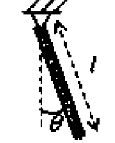
\includegraphics[width=0.6\textwidth]{4.png}
    \caption{}
    \label{fig:question28}
\end{figure}
    
\begin{multicols}{4}
\begin{enumerate}
\item $\sqrt{\frac{g}{2l}}$
\item $\sqrt{\frac{g}{l}}$
\item $\sqrt{\frac{2g}{l}}$
\item $\sqrt{\frac{3g}{2l}}$
\end{enumerate}
\end{multicols}
\hfill (GATE AE 2010)

\item The thin rectangular plate shown in the figure is loaded with uniform shear, $\tau_0$, along all edges and uniform uniaxial tension in the y-direction. The appropriate Airy's stress function to solve for stresses is given by
\begin{figure}[H]
    \centering
    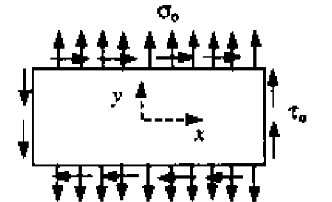
\includegraphics[width=0.6\textwidth]{5.png}
    \caption{}
    \label{fig:question29}
\end{figure}

\begin{multicols}{2}
\begin{enumerate}
\item $-\tau_{\alpha}xy - \sigma_{\alpha}\frac{x^2}{2} + \sigma_{\alpha}(x^4 - y^4)$
\item $\tau_{\alpha}xy - \sigma_{\alpha}\frac{x^2}{2}$
\item $-\tau_{\alpha}xy + \sigma_{\alpha}\frac{x^2}{2}$
\item $\tau_{\alpha}xy + \sigma_{\alpha}\frac{x^2}{2} + \sigma_{\alpha}(x^4 - y^4)$
\end{enumerate}
\end{multicols}
\hfill (GATE AE 2010)

\item A propeller powered aircraft, trimmed to attain maximum range and flying in a straight line, travels a distance $R$ from its take-off point when it has consumed a weight of fuel equal to $20\%$ of its take-off weight. If the aircraft continues to fly and consumes a total weight of fuel equal to $50\%$ of its take-off weight, the distance between it and its take-off point becomes:

\begin{multicols}{4}
\begin{enumerate}
\item $2.5R$  
\item $3.1R$  
\item $2.1R$  
\item $3.9R$  
\end{enumerate}
\end{multicols}
\hfill (GATE AE 2010)

\item The given thin wall section of uniform thickness, $t$, is symmetric about x-axis. Moment of inertia is given to be $I_{xx} = \frac{35}{12} t h^3$. Shear center for this section is located at:

\begin{figure}[H]
\centering
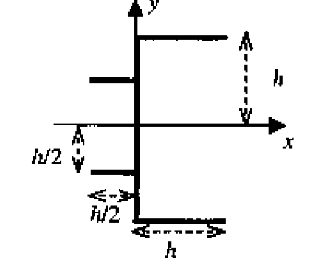
\includegraphics[width=0.6\textwidth]{6.png}
\caption{}
\label{fig:question31}
\end{figure}

\begin{multicols}{4}
\begin{enumerate}
\item $x = \frac{3}{8} h$  
\item $x = \frac{9}{28} h$  
\item $x = \frac{35}{36} h$  
\item $x = \frac{17}{35} h$  
\end{enumerate}
\end{multicols}
\hfill (GATE AE 2010)

\item During an under-damped oscillation of a single degree of freedom system, in the time-displacement plot the third peak is of magnitude $100$ and the tenth peak is of magnitude $10$. The damping ratio $\zeta$ is approximately:

\begin{multicols}{4}
\begin{enumerate}
\item $0.052$  
\item $0.023$  
\item $0.366$  
\item $0.159$  
\end{enumerate}
\end{multicols}
\hfill (GATE AE 2010)

\item Given that the Laplace transform of $y(t) = e^{-t} (2 \cos 2t - \sin 2t)$ is $Y(s) = \frac{2s}{(s + 1)^2 + 4}$, the Laplace transform of $y_t(t) = e^t (2 \cos 2t - \sin 2t)$ is:

\begin{multicols}{4}
\begin{enumerate}
\item $\frac{2(s - 2)}{(s - 1)^2 + 4}$  
\item $\frac{2(s + 2)}{(s + 3)^2 + 4}$  
\item $\frac{2(s + 2)}{(s + 1)^2 + 4}$  
\item $\frac{2(s - 1)}{(s - 1)^2 + 4}$  
\end{enumerate}
\end{multicols}
\hfill (GATE AE 2010)

\item In a certain region a hill is described by the shape $z(x,y) = \frac{1}{50} x^4 + y^3 - xy - 3y$, where the axes $x$ and $y$ are in the horizontal plane and axis $z$ points vertically upward. If $\hat{i}$, $\hat{j}$ and $\hat{k}$ are unit vectors along $x$, $y$ and $z$, respectively, then at the point $x = 5$, $y = 10$ the unit vector in the direction of the steepest slope of the hill will be:

\begin{multicols}{4}
\begin{enumerate}
\item $\hat{i}$  
\item $\hat{j}$  
\item $\hat{k}$  
\item $\hat{i} + \hat{j} + \hat{k}$  
\end{enumerate}
\end{multicols}
\hfill (GATE AE 2010)

\item An aircraft is cruising at an altitude of $9$ km. The free-stream static pressure and density at this altitude are $3.08 \times 10^4$ N/m$^2$ and $0.467$ kg/m$^3$ respectively. A Pitot tube mounted on the wing senses a pressure of $3.31 \times 10^4$ N/m$^2$. Ignoring compressibility effects, the cruising speed of the aircraft is approximately:

\begin{multicols}{4}
\begin{enumerate}
\item $50$ m/s  
\item $100$ m/s  
\item $150$ m/s  
\item $200$ m/s  
\end{enumerate}
\end{multicols}
\hfill (GATE AE 2010)

\item The trim curves of an aircraft are of the form $ C_{m, i} = (0.05 - 0.2 \delta_i) - 0.1C_L $ where the elevator deflection angle, $\delta_i$, is in radians. The static margin of the aircraft is:
\begin{multicols}{4}
\begin{enumerate}
\item 0.5
\item 0.2
\item 0.1
\item 0.05
\end{enumerate}
\end{multicols}
\hfill (GATE AE 2010)

\item The function $ f(x, y) = x^2 + y^2 - xy - 3y $ has an extremum at the point
\begin{multicols}{4}
\begin{enumerate}
\item (1.2)
\item (3.0)
\item (2.2)
\item (1.1)
\end{enumerate}
\end{multicols}
\hfill (GATE AE 2010)

\item Consider the flow of air ($ \rho = 1.23  \text{kg/m}^3 $) over a wing of chord length 0.5 m and span 3 m. Let the free stream velocity be $ U = 100  \text{m/s} $ and the average circulation around the wing be $ \Gamma = 10  \text{m}^2/\text{s} $ per unit span. The lift force acting on the wing is
\begin{multicols}{4}
\begin{enumerate}
\item 615 N
\item 1845 N
\item 3690 N
\item 4920 N
\end{enumerate}
\end{multicols}
\hfill (GATE AE 2010)

\item The stagnation pressure and stagnation temperature inside the combustion chamber of a liquid rocket engine are 1.5 MPa and 2500 K respectively. The burned gases have $ \gamma = 1.2 $ and $ R = 692.83  \text{J/kgK} $. The rocket has a converging - diverging nozzle with a throat area of 0.025 $ \text{m}^2 $ and the flow at the exit of the nozzle is supersonic. If the flow through the nozzle is isentropic, what is the mass flow rate of the gases out of the nozzle?
\begin{multicols}{4}
\begin{enumerate}
\item 18.5 kg/s
\item 31.2 kg/s
\item 29.7 kg/s
\item 19.4 kg/s
\end{enumerate}
\end{multicols}
\hfill (GATE AE 2010)

\item In finding a root of the equation: $ x^2 - 6x + 5 = 0 $ the Newton-Raphson method achieves an order of convergence equal to:
\begin{multicols}{4}
\begin{enumerate}
\item 1.0
\item 1.67
\item 2.0
\item 2.5
\end{enumerate}
\end{multicols}
\hfill (GATE AE 2010)

\item Consider a 1-D adiabatic, inviscid, compressible flow of air ($ R = 287  \text{J/Kg-K}, c_v = 718  \text{J/Kg-K} $) through a duct of constant cross-sectional area $ A = 1  \text{m}^2 $. If the volumetric flow rate is $ Q = 680  \text{m}^3/\text{s} $ and stagnation temperature is $ T_0 = 580.05  \text{K} $, then the air temperature inside the duct is
\begin{multicols}{4}
\begin{enumerate}
\item 300 K
\item 350 K
\item 400 K
\item 450 K
\end{enumerate}
\end{multicols}
\hfill (GATE AE 2010)

\item A two stage chemical rocket, having the same specific impulse ($ t_{ip} $) of 300 s for both the stages is designed in such a way that the payload ratio and the structural ratio are same for both the stages. The second stage of the rocket has following mass distribution:
    
    Propellant Mass = 10208 kg 
    
    Structural Mass = 1134 kg 
    
    Payload Mass = 1700 kg 
    
    $ g_e = 9.8  \text{m/s}^2 $ 
    
    If the rocket is fired from rest and it flies in a zero gravity field and a drag free environment, the final velocity attained by the payload is
\begin{multicols}{4}
\begin{enumerate}
\item 9729.3 m/s
\item 897.3 m/s
\item 9360.2 m/s
\item 8973.2 m/s
\end{enumerate}
\end{multicols}
\hfill (GATE AE 2010)

\item A missile with a Ramjet engine is flying in air. The temperature at the inlet and the outlet of the combustor are 1200 K and 2500 K respectively. The heating value of the fuel is 43 MJ/kg and the burner efficiency is 90\%. Considering the working fluid to be air ($ C_P = 1005  \text{J/kgK} $ and $ \gamma = 1.4 $), the fuel/air ratio ($ f = \frac{m_f}{m_a} $) for this engine is equal to:
\begin{multicols}{4}
\begin{enumerate}
\item 0.032
\item 0.036
\item 0.042
\item 0.026
\end{enumerate}
\end{multicols}
\hfill (GATE AE 2010)

\item The trim curves of an aircraft are of the form $ C_{m_{v,i}} = (0.05 - 0.2 \delta_r) - 0.1C_t $ where the elevator deflection angle, $\delta_r$, is in radians. The change in elevator deflection needed to increase the lift coefficient from 0.4 to 0.9 is:
\begin{multicols}{4}
\begin{enumerate}
\item $-0.5$ radians
\item $-0.25$ radians
\item 0.25 radians
\item 0.5 radians
\end{enumerate}
\end{multicols}
\hfill (GATE AE 2010)

\item If e is the base of the natural logarithms then the equation of the tangent from the origin to the curve $ y = e^x $ is
\begin{multicols}{4}
\begin{enumerate}
\item $ y = x $
\item $ y = \pi x $
\item $ y = \frac{x}{e} $
\item $ y = ex $
\end{enumerate}
\end{multicols}
\hfill (GATE AE 2010)

\item Consider a potential flow over a finite wing with the following circulation distribution
    $\Gamma(y) = 100 \sqrt{1 - \left( \frac{2y}{4} \right)^2 m^2 / s}$ 
    
    \begin{figure}[H]
\centering
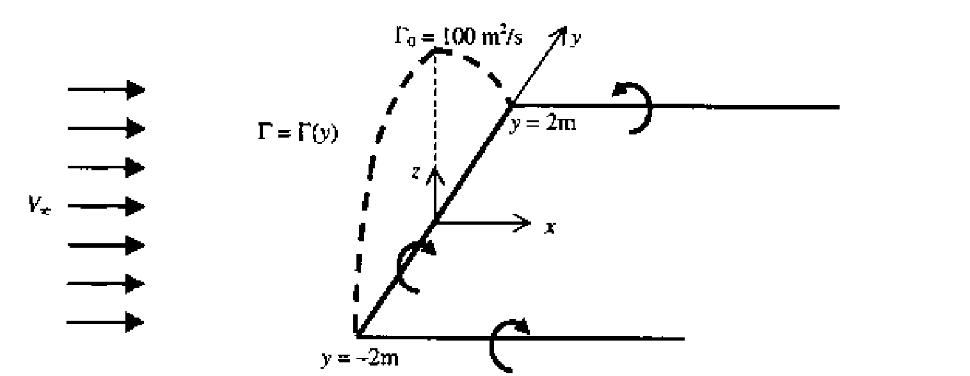
\includegraphics[width=0.6\textwidth]{7.png}
\caption{Thin-walled symmetric section}
\label{fig:question46}
\end{figure}

    If the free stream velocity is 100 m/s, the induced angle of attack is
\begin{multicols}{2}
\begin{enumerate}
\item 0.125 radians
\item $-0.125$ radians
\item $ 0.125 \sqrt{1 - \left( \frac{y}{2} \right)^2}$ radians
\item $-0.125 \sqrt{1 - \left( \frac{y}{2} \right)^2}$ radians
\end{enumerate}
\end{multicols}
\hfill (GATE AE 2010)

\item The inlet stagnation temperature for a single stage axial compressor is 300 K and the stage efficiency is 0.80. Following conditions exist at the mean radius of the rotor blade: 

    Blade speed = 200 m/s 
    
    Axial flow velocity = 160 m/s 
    
    Inlet blade angle $\beta_1 = 44^\circ$ 
    
    Outlet blade angle $\beta_2 = 14^\circ$ 
    
    $ C_p = 1005  J/kgK $ and $\gamma = 1.4$ 
    
    What is the stagnation pressure ratio ($ P_{RE} $) for this compressor?
\begin{multicols}{4}
\begin{enumerate}
\item 1.41
\item 1.37
\item 1.51
\item 1.23
\end{enumerate}
\end{multicols}
\hfill (GATE AE 2010)

\textbf{Common Data Questions}

\textbf{Common Data for Questions 48 and 49:}

    Consider a simply supported beam of length $ L $, carrying a bracket welded at its center. The bracket carries a vertical load, $ P $, as shown in the figure. Dimensions of bracket are $ a = 0.1L $. The beam has a square cross section of dimension $ h \times h $.

\begin{figure}[H]
\centering
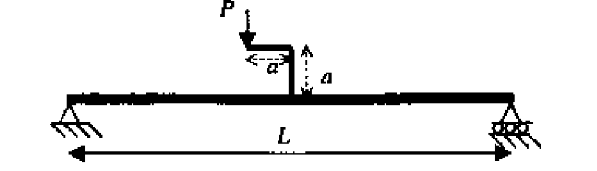
\includegraphics[width=0.5\textwidth]{8.png}
\caption{Thin-walled symmetric section}
\label{fig:question48,49}
\end{figure}

\item Bending moment diagram is given by
\begin{enumerate}
    \item 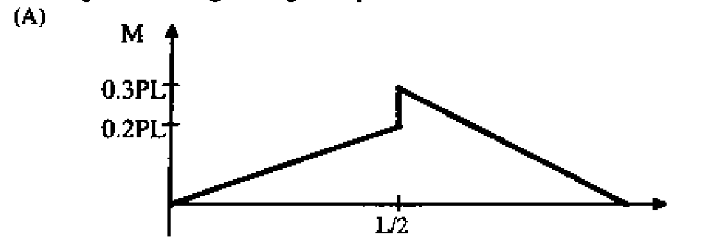
\includegraphics[width=0.2\textwidth]{9.png}
    \item 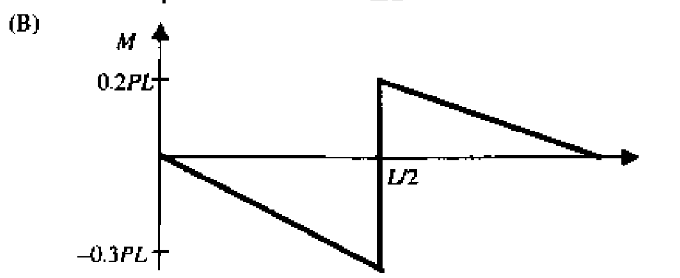
\includegraphics[width=0.2\textwidth]{10.png}
    \item 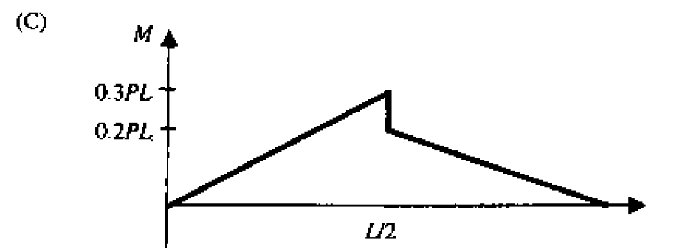
\includegraphics[width=0.2\textwidth]{11.png}
    \item 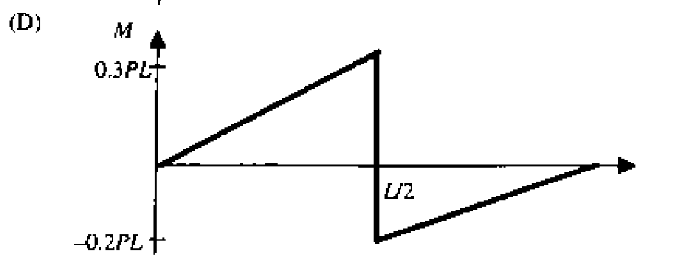
\includegraphics[width=0.2\textwidth]{12.png}
\end{enumerate}
\hfill (GATE AE 2010)

\item Maximum value of shear stress is
\begin{multicols}{4}
\begin{enumerate}
\item 0.67 $ P/h^2 $
\item 1.33 $ P/h^2 $
\item 1.5 $ P/h^2 $
\item 0.9 $ P/h^2 $
\end{enumerate}
\end{multicols}
\hfill (GATE AE 2010)

\textbf{Common Data for Questions 50 and 51:}
    Consider a potential flow over a spinning cylinder. The stream function is given as

\begin{figure}[H]
\centering
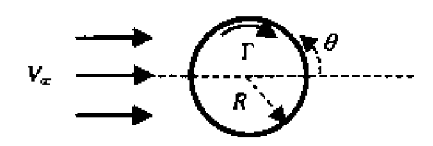
\includegraphics[width=0.5\textwidth]{13.png}
\caption{Thin-walled symmetric section}
\label{fig:question48,49}
\end{figure}

    $ \psi = (V_a r \sin \theta)(1 - \frac{R^2}{r^2}) + \frac{\Gamma}{2\pi} \ln \frac{r}{R} $ 
    
    where 
    
    Free stream velocity, $ V_a = 25  m/s $ 
    
    Cylinder radius, $ R = 1  m $ 
    
    Circulation, $ \Gamma = 50\pi  m^2/s $ 
    
\item The radial and azimuthal velocities on the cylinder surface at $ \theta = \pi / 2  are $ 
\begin{multicols}{2}
\begin{enumerate}
\item $ V_r = 0  m/s $, $ V_\theta = -75  m/s $
\item $ V_r = 0  m/s $, $ V_\theta = 75  m/s $
\item $ V_r = 0  m/s $, $ V_\theta = -25  m/s $
\item $ V_r = 0  m/s $, $ V_\theta = 25  m/s $
\end{enumerate}
\end{multicols}
\hfill (GATE AE 2010)

\item The stagnation points are located at
\begin{multicols}{4}
\begin{enumerate}
\item $ 210^\circ $ and $ 330^\circ $
\item $ 240^\circ $ and $ 300^\circ $
\item $ 30^\circ $ and $ 150^\circ $
\item $ 60^\circ $ and $ 120^\circ $
\end{enumerate}
\end{multicols}
\hfill (GATE AE 2010)

\textbf{Linked Answer Questions}

\textbf{Statement for Linked Answer Questions 52 and 53:}

    An aircraft with an IDEAL Turbojet engine is flying at 200 m/s at an altitude where the ambient pressure is equal to 0.8 bar. The stagnation pressure and temperature at the inlet of the turbine are 6 bar and 1400 K respectively. The change in specific enthalpy across the compressor is 335 kJ/kg. Assume the fuel flow rate to be very small in comparison to the air flow rate and consider $ C_p = 1117  J/kgK $ and $ \gamma = 1.3 $.
    
\item What is the stagnation pressure at the inlet of the nozzle?
\begin{multicols}{4}
\begin{enumerate}
\item 2.8 bar
\item 5.7 bar
\item 2.1 bar
\item 6.3 bar
\end{enumerate}
\end{multicols}
\hfill (GATE AE 2010)

\item What is the specific thrust produced by this engine under the given conditions?
\begin{multicols}{4}
\begin{enumerate}
\item 586 Ns/kg
\item 745 Ns/kg
\item 686 Ns/kg
\item 500 Ns/kg
\end{enumerate}
\end{multicols}
\hfill (GATE AE 2010)

\textbf{Statement for Linked Answer Questions 54 and 55:}

    An aircraft is in straight and level flight at a constant speed v. It is disturbed by a symmetric vertical gust, resulting in a plugoid oscillation of time period $ T $.
    
\item Assuming that g is the acceleration due to gravity, $ T $ is given approximately by:
\begin{multicols}{4}
\begin{enumerate}
\item $ \frac{v}{\pi g} $
\item $ \frac{\pi v}{g} $
\item $ \frac{v}{\sqrt{2}\pi g} $
\item $ \frac{\sqrt{2}\pi v}{g} $
\end{enumerate}
\end{multicols}
\hfill (GATE AE 2010)

\item If $ v = 200  m/s $ then the wavelength of the plugoid oscillations, assuming $ g = 9.81  m/s^2 $, is, approximately:
\begin{multicols}{4}
\begin{enumerate}
\item $ 1.28 \times 10^4  m $
\item $ 1.30 \times 10^3  m $
\item $ 1.81 \times 10^4  m $
\item $ 918  m $
\end{enumerate}
\end{multicols}
\hfill (GATE AE 2010)

\textbf{General Aptitude (GA) Questions}

\item \textit{Which of the following options is the closest in meaning to the word below:}

\textbf{Circulious}

\begin{enumerate}
\item cyclic
\item indirect
\item confusing
\item crooked
\end{enumerate}
\hfill (GATE AE 2010)

\item \textit{The question below consists of a pair of related words followed by four pairs of words. Select the pair that best expresses the relation in the original pair.}

\textbf{Unemployed : Worker}

\begin{enumerate}
\item fallow : land
\item unaware : sleeper
\item wit : jester
\item renovated : house
\end{enumerate}
\hfill (GATE AE 2010)

\item \textit{Choose the most appropriate word from the options given below to complete the following sentence:}

\textbf{If we manage to ------------ our natural resources, we would leave a better planet for our children.}

\begin{enumerate}
\item uphold
\item restrain
\item cherish
\item conserve
\end{enumerate}
\hfill (GATE AE 2010)

\item \textit{Choose the most appropriate word from the options given below to complete the following sentence:}

\textbf{His rather casual remarks on politics ------------ his lack of seriousness about the subject.}

\begin{enumerate}
\item masked
\item belied
\item betrayed
\item suppressed
\end{enumerate}
\hfill (GATE AE 2010)

\item 25 persons are in a room. 15 of them play hockey, 17 of them play football and 10 of them play both hockey and football. Then the number of persons playing neither hockey nor football is:
\begin{multicols}{4}
\begin{enumerate}
\item 2
\item 17
\item 13
\item 3
\end{enumerate}
\end{multicols}
\hfill (GATE AE 2010)

\item \textbf{Modern warfare has changed from large scale clashes of armies to suppression of civilian populations. Chemical agents that do their work silently appear to be suited to such warfare; and regretfully, there exist people in military establishments who think that chemical agents are useful tools for their cause.}
    
\textit{Which of the following statements best sums up the meaning of the above passage:}

\begin{enumerate}
\item Modern warfare has resulted in civil strife.
\item Chemical agents are useful in modern warfare.
\item Use of chemical agents in warfare would be undesirable.
\item People in military establishments like to use chemical agents in war.
\end{enumerate}
\hfill (GATE AE 2010)

\item If 137 + 276 = 435 how much is 731 + 672?
\begin{multicols}{4}
\begin{enumerate}
\item 534
\item 1403
\item 1623
\item 1513
\end{enumerate}
\end{multicols}
\hfill (GATE AE 2010)

\item 5 skilled workers can build a wall in 20 days; 8 semi-skilled workers can build a wall in 25 days; 10 unskilled workers can build a wall in 30 days. If a team has 2 skilled, 6 semi-skilled and 5 unskilled workers, how long will it take to build the wall?
\begin{multicols}{4}
\begin{enumerate}
\item 20 days
\item 18 days
\item 16 days
\item 15 days
\end{enumerate}
\end{multicols}
\hfill (GATE AE 2010)

\item Given digits 2, 2, 3, 3, 3, 4, 4, 4, 4 how many distinct 4 digit numbers greater than 3000 can be formed?
\begin{multicols}{4}
\begin{enumerate}
\item 50
\item 51
\item 52
\item 54
\end{enumerate}
\end{multicols}
\hfill (GATE AE 2010)

\item Hari (H), Gita (G), Irfan (I) and Saira (S) are siblings (i.e. brothers and sisters). All were born on 1st January. The age difference between any two successive siblings (that is born one after another) is less than 3 years. Given the following facts: 

    i. Hari's age + Gita's age > Irfan's age + Saira's age. 
    
    ii. The age difference between Gita and Saira is 1 year. However, Gita is not the oldest and Saira is not the youngest. 
    
    iii. There are no twins. 
    
    In what order were they born (oldest first)?
\begin{multicols}{4}
\begin{enumerate}
\item HSIG
\item SGHI
\item IGSH
\item IHSG
\end{enumerate}
\end{multicols}
\hfill (GATE AE 2010)

\end{enumerate}
\end{document}
